\documentclass[1p]{elsarticle_modified}
%\bibliographystyle{elsarticle-num}

%\usepackage[colorlinks]{hyperref}
%\usepackage{abbrmath_seonhwa} %\Abb, \Ascr, \Acal ,\Abf, \Afrak
\usepackage{amsfonts}
\usepackage{amssymb}
\usepackage{amsmath}
\usepackage{amsthm}
\usepackage{scalefnt}
\usepackage{amsbsy}
\usepackage{kotex}
\usepackage{caption}
\usepackage{subfig}
\usepackage{color}
\usepackage{graphicx}
\usepackage{xcolor} %% white, black, red, green, blue, cyan, magenta, yellow
\usepackage{float}
\usepackage{setspace}
\usepackage{hyperref}

\usepackage{tikz}
\usetikzlibrary{arrows}

\usepackage{multirow}
\usepackage{array} % fixed length table
\usepackage{hhline}

%%%%%%%%%%%%%%%%%%%%%
\makeatletter
\renewcommand*\env@matrix[1][\arraystretch]{%
	\edef\arraystretch{#1}%
	\hskip -\arraycolsep
	\let\@ifnextchar\new@ifnextchar
	\array{*\c@MaxMatrixCols c}}
\makeatother %https://tex.stackexchange.com/questions/14071/how-can-i-increase-the-line-spacing-in-a-matrix
%%%%%%%%%%%%%%%

\usepackage[normalem]{ulem}

\newcommand{\msout}[1]{\ifmmode\text{\sout{\ensuremath{#1}}}\else\sout{#1}\fi}
%SOURCE: \msout is \stkout macro in https://tex.stackexchange.com/questions/20609/strikeout-in-math-mode

\newcommand{\cancel}[1]{
	\ifmmode
	{\color{red}\msout{#1}}
	\else
	{\color{red}\sout{#1}}
	\fi
}

\newcommand{\add}[1]{
	{\color{blue}\uwave{#1}}
}

\newcommand{\replace}[2]{
	\ifmmode
	{\color{red}\msout{#1}}{\color{blue}\uwave{#2}}
	\else
	{\color{red}\sout{#1}}{\color{blue}\uwave{#2}}
	\fi
}

\newcommand{\Sol}{\mathcal{S}} %segment
\newcommand{\D}{D} %diagram
\newcommand{\A}{\mathcal{A}} %arc


%%%%%%%%%%%%%%%%%%%%%%%%%%%%%5 test

\def\sl{\operatorname{\textup{SL}}(2,\Cbb)}
\def\psl{\operatorname{\textup{PSL}}(2,\Cbb)}
\def\quan{\mkern 1mu \triangleright \mkern 1mu}

\theoremstyle{definition}
\newtheorem{thm}{Theorem}[section]
\newtheorem{prop}[thm]{Proposition}
\newtheorem{lem}[thm]{Lemma}
\newtheorem{ques}[thm]{Question}
\newtheorem{cor}[thm]{Corollary}
\newtheorem{defn}[thm]{Definition}
\newtheorem{exam}[thm]{Example}
\newtheorem{rmk}[thm]{Remark}
\newtheorem{alg}[thm]{Algorithm}

\newcommand{\I}{\sqrt{-1}}
\begin{document}

%\begin{frontmatter}
%
%\title{Boundary parabolic representations of knots up to 8 crossings}
%
%%% Group authors per affiliation:
%\author{Yunhi Cho} 
%\address{Department of Mathematics, University of Seoul, Seoul, Korea}
%\ead{yhcho@uos.ac.kr}
%
%
%\author{Seonhwa Kim} %\fnref{s_kim}}
%\address{Center for Geometry and Physics, Institute for Basic Science, Pohang, 37673, Korea}
%\ead{ryeona17@ibs.re.kr}
%
%\author{Hyuk Kim}
%\address{Department of Mathematical Sciences, Seoul National University, Seoul 08826, Korea}
%\ead{hyukkim@snu.ac.kr}
%
%\author{Seokbeom Yoon}
%\address{Department of Mathematical Sciences, Seoul National University, Seoul, 08826,  Korea}
%\ead{sbyoon15@snu.ac.kr}
%
%\begin{abstract}
%We find all boundary parabolic representation of knots up to 8 crossings.
%
%\end{abstract}
%\begin{keyword}
%    \MSC[2010] 57M25 
%\end{keyword}
%
%\end{frontmatter}

%\linenumbers
%\tableofcontents
%
\newcommand\colored[1]{\textcolor{white}{\rule[-0.35ex]{0.8em}{1.4ex}}\kern-0.8em\color{red} #1}%
%\newcommand\colored[1]{\textcolor{white}{ #1}\kern-2.17ex	\textcolor{white}{ #1}\kern-1.81ex	\textcolor{white}{ #1}\kern-2.15ex\color{red}#1	}

{\Large $\underline{12a_{0548}~(K12a_{0548})}$}

\setlength{\tabcolsep}{10pt}
\renewcommand{\arraystretch}{1.6}
\vspace{1cm}\begin{tabular}{m{100pt}>{\centering\arraybackslash}m{274pt}}
\multirow{5}{120pt}{
	\centering
	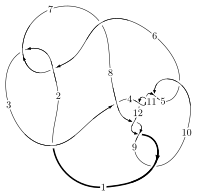
\includegraphics[width=112pt]{../../../GIT/diagram.site/Diagrams/png/1349_12a_0548.png}\\
\ \ \ A knot diagram\footnotemark}&
\allowdisplaybreaks
\textbf{Linearized knot diagam} \\
\cline{2-2}
 &
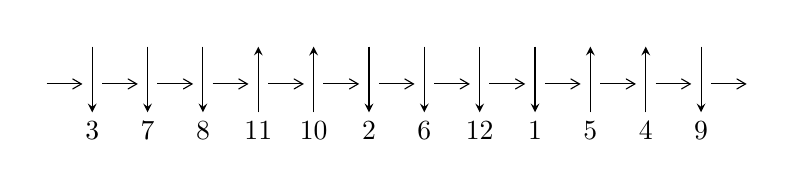
\begin{tikzpicture}[x=20pt, y=17pt]
	% nodes
	\node (C0) at (0, 0) {};
	\node (C1) at (1, 0) {};
	\node (C1U) at (1, +1) {};
	\node (C1D) at (1, -1) {3};

	\node (C2) at (2, 0) {};
	\node (C2U) at (2, +1) {};
	\node (C2D) at (2, -1) {7};

	\node (C3) at (3, 0) {};
	\node (C3U) at (3, +1) {};
	\node (C3D) at (3, -1) {8};

	\node (C4) at (4, 0) {};
	\node (C4U) at (4, +1) {};
	\node (C4D) at (4, -1) {11};

	\node (C5) at (5, 0) {};
	\node (C5U) at (5, +1) {};
	\node (C5D) at (5, -1) {10};

	\node (C6) at (6, 0) {};
	\node (C6U) at (6, +1) {};
	\node (C6D) at (6, -1) {2};

	\node (C7) at (7, 0) {};
	\node (C7U) at (7, +1) {};
	\node (C7D) at (7, -1) {6};

	\node (C8) at (8, 0) {};
	\node (C8U) at (8, +1) {};
	\node (C8D) at (8, -1) {12};

	\node (C9) at (9, 0) {};
	\node (C9U) at (9, +1) {};
	\node (C9D) at (9, -1) {1};

	\node (C10) at (10, 0) {};
	\node (C10U) at (10, +1) {};
	\node (C10D) at (10, -1) {5};

	\node (C11) at (11, 0) {};
	\node (C11U) at (11, +1) {};
	\node (C11D) at (11, -1) {4};

	\node (C12) at (12, 0) {};
	\node (C12U) at (12, +1) {};
	\node (C12D) at (12, -1) {9};
	\node (C13) at (13, 0) {};

	% arrows
	\draw[->,>={angle 60}]
	(C0) edge (C1) (C1) edge (C2) (C2) edge (C3) (C3) edge (C4) (C4) edge (C5) (C5) edge (C6) (C6) edge (C7) (C7) edge (C8) (C8) edge (C9) (C9) edge (C10) (C10) edge (C11) (C11) edge (C12) (C12) edge (C13) ;	\draw[->,>=stealth]
	(C1U) edge (C1D) (C2U) edge (C2D) (C3U) edge (C3D) (C4D) edge (C4U) (C5D) edge (C5U) (C6U) edge (C6D) (C7U) edge (C7D) (C8U) edge (C8D) (C9U) edge (C9D) (C10D) edge (C10U) (C11D) edge (C11U) (C12U) edge (C12D) ;
	\end{tikzpicture} \\
\hhline{~~} \\& 
\textbf{Solving Sequence} \\ \cline{2-2} 
 &
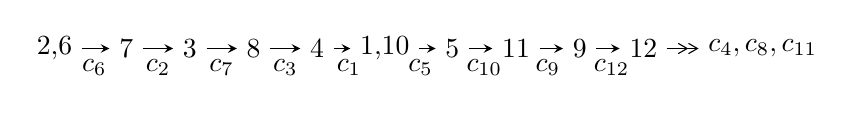
\begin{tikzpicture}[x=23pt, y=7pt]
	% node
	\node (A0) at (-1/8, 0) {2,6};
	\node (A1) at (1, 0) {7};
	\node (A2) at (2, 0) {3};
	\node (A3) at (3, 0) {8};
	\node (A4) at (4, 0) {4};
	\node (A5) at (81/16, 0) {1,10};
	\node (A6) at (49/8, 0) {5};
	\node (A7) at (57/8, 0) {11};
	\node (A8) at (65/8, 0) {9};
	\node (A9) at (73/8, 0) {12};
	\node (C1) at (1/2, -1) {$c_{6}$};
	\node (C2) at (3/2, -1) {$c_{2}$};
	\node (C3) at (5/2, -1) {$c_{7}$};
	\node (C4) at (7/2, -1) {$c_{3}$};
	\node (C5) at (9/2, -1) {$c_{1}$};
	\node (C6) at (45/8, -1) {$c_{5}$};
	\node (C7) at (53/8, -1) {$c_{10}$};
	\node (C8) at (61/8, -1) {$c_{9}$};
	\node (C9) at (69/8, -1) {$c_{12}$};
	\node (A10) at (11, 0) {$c_{4},c_{8},c_{11}$};

	% edge
	\draw[->,>=stealth]	
	(A0) edge (A1) (A1) edge (A2) (A2) edge (A3) (A3) edge (A4) (A4) edge (A5) (A5) edge (A6) (A6) edge (A7) (A7) edge (A8) (A8) edge (A9) ;
	\draw[->>,>={angle 60}]	
	(A9) edge (A10);
\end{tikzpicture} \\ 

\end{tabular} \\

\footnotetext{
The image of knot diagram is generated by the software ``\textbf{Draw programme}" developed by Andrew Bartholomew(\url{http://www.layer8.co.uk/maths/draw/index.htm\#Running-draw}), where we modified some parts for our purpose(\url{https://github.com/CATsTAILs/LinksPainter}).
}\phantom \\ \newline 
\centering \textbf{Ideals for irreducible components\footnotemark of $X_{\text{par}}$} 
 
\begin{align*}
I^u_{1}&=\langle 
-1.58134\times10^{20} u^{62}+3.74205\times10^{20} u^{61}+\cdots+2.91973\times10^{21} b-2.96150\times10^{21},\\
\phantom{I^u_{1}}&\phantom{= \langle  }-1.26309\times10^{22} u^{62}+1.69902\times10^{22} u^{61}+\cdots+8.75918\times10^{21} a-5.81824\times10^{22},\;u^{63}-2 u^{62}+\cdots+5 u-3\rangle \\
I^u_{2}&=\langle 
- u^2 a- a u- u^2+b- u-1,\;a^2+2 a u+3 u^2+2 a+2 u+1,\;u^3+u^2-1\rangle \\
I^u_{3}&=\langle 
b,\;a- u+1,\;u^3- u^2+1\rangle \\
\\
\end{align*}
\raggedright * 3 irreducible components of $\dim_{\mathbb{C}}=0$, with total 72 representations.\\
\footnotetext{All coefficients of polynomials are rational numbers. But the coefficients are sometimes approximated in decimal forms when there is not enough margin.}
\newpage
\renewcommand{\arraystretch}{1}
\centering \section*{I. $I^u_{1}= \langle -1.58\times10^{20} u^{62}+3.74\times10^{20} u^{61}+\cdots+2.92\times10^{21} b-2.96\times10^{21},\;-1.26\times10^{22} u^{62}+1.70\times10^{22} u^{61}+\cdots+8.76\times10^{21} a-5.82\times10^{22},\;u^{63}-2 u^{62}+\cdots+5 u-3 \rangle$}
\flushleft \textbf{(i) Arc colorings}\\
\begin{tabular}{m{7pt} m{180pt} m{7pt} m{180pt} }
\flushright $a_{2}=$&$\begin{pmatrix}0\\u\end{pmatrix}$ \\
\flushright $a_{6}=$&$\begin{pmatrix}1\\0\end{pmatrix}$ \\
\flushright $a_{7}=$&$\begin{pmatrix}1\\u^2\end{pmatrix}$ \\
\flushright $a_{3}=$&$\begin{pmatrix}- u\\- u^3+u\end{pmatrix}$ \\
\flushright $a_{8}=$&$\begin{pmatrix}- u^2+1\\u^2\end{pmatrix}$ \\
\flushright $a_{4}=$&$\begin{pmatrix}u^7-2 u^5+2 u^3-2 u\\- u^7+u^5-2 u^3+u\end{pmatrix}$ \\
\flushright $a_{1}=$&$\begin{pmatrix}u^3\\u^5- u^3+u\end{pmatrix}$ \\
\flushright $a_{10}=$&$\begin{pmatrix}1.44202 u^{62}-1.93971 u^{61}+\cdots+0.661158 u+6.64244\\0.0541605 u^{62}-0.128165 u^{61}+\cdots-0.441955 u+1.01431\end{pmatrix}$ \\
\flushright $a_{5}=$&$\begin{pmatrix}-0.185702 u^{62}+0.0752726 u^{61}+\cdots-2.14838 u+0.547461\\0.719076 u^{62}-0.662451 u^{61}+\cdots-0.943387 u+1.09817\end{pmatrix}$ \\
\flushright $a_{11}=$&$\begin{pmatrix}0.903442 u^{62}-1.53591 u^{61}+\cdots+1.76710 u+4.49679\\-0.804672 u^{62}+1.13906 u^{61}+\cdots+1.28977 u-3.03093\end{pmatrix}$ \\
\flushright $a_{9}=$&$\begin{pmatrix}1.18523 u^{62}-1.75085 u^{61}+\cdots+1.47609 u+5.39500\\-0.563042 u^{62}+0.514494 u^{61}+\cdots+0.795969 u-0.856839\end{pmatrix}$ \\
\flushright $a_{12}=$&$\begin{pmatrix}0.905223 u^{62}-1.45026 u^{61}+\cdots+0.887446 u+4.18778\\-0.569552 u^{62}+0.745346 u^{61}+\cdots+1.44587 u-2.47512\end{pmatrix}$\\&\end{tabular}
\flushleft \textbf{(ii) Obstruction class $= -1$}\\~\\
\flushleft \textbf{(iii) Cusp Shapes $= \frac{7126225419678175524155}{1459863554716009717429} u^{62}-\frac{8012124561236711506684}{1459863554716009717429} u^{61}+\cdots-\frac{14448360873832908916690}{1459863554716009717429} u+\frac{13917590278743478982007}{1459863554716009717429}$}\\~\\
\newpage\renewcommand{\arraystretch}{1}
\flushleft \textbf{(iv) u-Polynomials at the component}\newline \\
\begin{tabular}{m{50pt}|m{274pt}}
Crossings & \hspace{64pt}u-Polynomials at each crossing \\
\hline $$\begin{aligned}c_{1},c_{7}\end{aligned}$$&$\begin{aligned}
&u^{63}+22 u^{62}+\cdots+79 u+9
\end{aligned}$\\
\hline $$\begin{aligned}c_{2},c_{6}\end{aligned}$$&$\begin{aligned}
&u^{63}-2 u^{62}+\cdots+5 u-3
\end{aligned}$\\
\hline $$\begin{aligned}c_{3}\end{aligned}$$&$\begin{aligned}
&u^{63}+2 u^{62}+\cdots-2119 u-507
\end{aligned}$\\
\hline $$\begin{aligned}c_{4},c_{5},c_{10}\\c_{11}\end{aligned}$$&$\begin{aligned}
&u^{63}- u^{62}+\cdots-32 u-8
\end{aligned}$\\
\hline $$\begin{aligned}c_{8},c_{9},c_{12}\end{aligned}$$&$\begin{aligned}
&u^{63}+4 u^{62}+\cdots+12 u-1
\end{aligned}$\\
\hline
\end{tabular}\\~\\
\newpage\renewcommand{\arraystretch}{1}
\flushleft \textbf{(v) Riley Polynomials at the component}\newline \\
\begin{tabular}{m{50pt}|m{274pt}}
Crossings & \hspace{64pt}Riley Polynomials at each crossing \\
\hline $$\begin{aligned}c_{1},c_{7}\end{aligned}$$&$\begin{aligned}
&y^{63}+42 y^{62}+\cdots-4037 y-81
\end{aligned}$\\
\hline $$\begin{aligned}c_{2},c_{6}\end{aligned}$$&$\begin{aligned}
&y^{63}-22 y^{62}+\cdots+79 y-9
\end{aligned}$\\
\hline $$\begin{aligned}c_{3}\end{aligned}$$&$\begin{aligned}
&y^{63}-30 y^{62}+\cdots+10968607 y-257049
\end{aligned}$\\
\hline $$\begin{aligned}c_{4},c_{5},c_{10}\\c_{11}\end{aligned}$$&$\begin{aligned}
&y^{63}+77 y^{62}+\cdots-384 y-64
\end{aligned}$\\
\hline $$\begin{aligned}c_{8},c_{9},c_{12}\end{aligned}$$&$\begin{aligned}
&y^{63}-64 y^{62}+\cdots-154 y-1
\end{aligned}$\\
\hline
\end{tabular}\\~\\
\newpage\flushleft \textbf{(vi) Complex Volumes and Cusp Shapes}
$$\begin{array}{c|c|c}  
\text{Solutions to }I^u_{1}& \I (\text{vol} + \sqrt{-1}CS) & \text{Cusp shape}\\
 \hline 
\begin{aligned}
u &= \phantom{-}0.610001 + 0.784154 I \\
a &= -0.583306 - 0.639284 I \\
b &= \phantom{-}0.10442 + 1.60088 I\end{aligned}
 & -6.01435 + 3.73785 I & -6.21764 - 2.33056 I \\ \hline\begin{aligned}
u &= \phantom{-}0.610001 - 0.784154 I \\
a &= -0.583306 + 0.639284 I \\
b &= \phantom{-}0.10442 - 1.60088 I\end{aligned}
 & -6.01435 - 3.73785 I & -6.21764 + 2.33056 I \\ \hline\begin{aligned}
u &= -0.691211 + 0.731938 I \\
a &= -0.984563 + 0.325099 I \\
b &= \phantom{-}0.423366 - 0.660007 I\end{aligned}
 & \phantom{-}1.70446 - 1.85626 I & -3.28574 + 4.17386 I \\ \hline\begin{aligned}
u &= -0.691211 - 0.731938 I \\
a &= -0.984563 - 0.325099 I \\
b &= \phantom{-}0.423366 + 0.660007 I\end{aligned}
 & \phantom{-}1.70446 + 1.85626 I & -3.28574 - 4.17386 I \\ \hline\begin{aligned}
u &= \phantom{-}0.984690 + 0.048731 I \\
a &= \phantom{-}0.390182 + 1.262910 I \\
b &= -0.214172 + 0.744109 I\end{aligned}
 & -3.63603 - 1.98289 I & -12.79221 + 5.30533 I \\ \hline\begin{aligned}
u &= \phantom{-}0.984690 - 0.048731 I \\
a &= \phantom{-}0.390182 - 1.262910 I \\
b &= -0.214172 - 0.744109 I\end{aligned}
 & -3.63603 + 1.98289 I & -12.79221 - 5.30533 I \\ \hline\begin{aligned}
u &= -0.617889 + 0.811854 I \\
a &= \phantom{-}1.21265 - 0.77110 I \\
b &= -0.569733 + 0.792616 I\end{aligned}
 & -4.01161 - 5.24201 I & -7.19231 + 3.97955 I \\ \hline\begin{aligned}
u &= -0.617889 - 0.811854 I \\
a &= \phantom{-}1.21265 + 0.77110 I \\
b &= -0.569733 - 0.792616 I\end{aligned}
 & -4.01161 + 5.24201 I & -7.19231 - 3.97955 I \\ \hline\begin{aligned}
u &= -0.800531 + 0.652431 I \\
a &= \phantom{-}0.356242 + 0.321397 I \\
b &= -0.225169 + 0.600163 I\end{aligned}
 & \phantom{-}0.12008 + 2.15047 I & -8.15527 - 1.56284 I \\ \hline\begin{aligned}
u &= -0.800531 - 0.652431 I \\
a &= \phantom{-}0.356242 - 0.321397 I \\
b &= -0.225169 - 0.600163 I\end{aligned}
 & \phantom{-}0.12008 - 2.15047 I & -8.15527 + 1.56284 I\\
 \hline 
 \end{array}$$\newpage$$\begin{array}{c|c|c}  
\text{Solutions to }I^u_{1}& \I (\text{vol} + \sqrt{-1}CS) & \text{Cusp shape}\\
 \hline 
\begin{aligned}
u &= -0.809657 + 0.514097 I \\
a &= \phantom{-}2.00737 + 1.05562 I \\
b &= -0.143570 - 1.274290 I\end{aligned}
 & -6.22882 + 2.00042 I & -11.28661 - 3.42546 I \\ \hline\begin{aligned}
u &= -0.809657 - 0.514097 I \\
a &= \phantom{-}2.00737 - 1.05562 I \\
b &= -0.143570 + 1.274290 I\end{aligned}
 & -6.22882 - 2.00042 I & -11.28661 + 3.42546 I \\ \hline\begin{aligned}
u &= \phantom{-}0.785085 + 0.714910 I \\
a &= -1.190430 + 0.036937 I \\
b &= \phantom{-}0.504608 - 0.222274 I\end{aligned}
 & \phantom{-}2.98803 - 1.39468 I & \phantom{-0.000000 } 0 \\ \hline\begin{aligned}
u &= \phantom{-}0.785085 - 0.714910 I \\
a &= -1.190430 - 0.036937 I \\
b &= \phantom{-}0.504608 + 0.222274 I\end{aligned}
 & \phantom{-}2.98803 + 1.39468 I & \phantom{-0.000000 } 0 \\ \hline\begin{aligned}
u &= \phantom{-}0.600448 + 0.711632 I \\
a &= \phantom{-}1.70429 + 0.06119 I \\
b &= -0.710743 + 0.153011 I\end{aligned}
 & -2.09343 + 0.92231 I & -4.75363 + 0.62378 I \\ \hline\begin{aligned}
u &= \phantom{-}0.600448 - 0.711632 I \\
a &= \phantom{-}1.70429 - 0.06119 I \\
b &= -0.710743 - 0.153011 I\end{aligned}
 & -2.09343 - 0.92231 I & -4.75363 - 0.62378 I \\ \hline\begin{aligned}
u &= \phantom{-}0.625396 + 0.875190 I \\
a &= \phantom{-}0.658938 + 1.166250 I \\
b &= -0.16972 - 1.64610 I\end{aligned}
 & -12.3245 + 8.0761 I & \phantom{-0.000000 } 0 \\ \hline\begin{aligned}
u &= \phantom{-}0.625396 - 0.875190 I \\
a &= \phantom{-}0.658938 - 1.166250 I \\
b &= -0.16972 + 1.64610 I\end{aligned}
 & -12.3245 - 8.0761 I & \phantom{-0.000000 } 0 \\ \hline\begin{aligned}
u &= -1.07798\phantom{ +0.000000I} \\
a &= -0.363979\phantom{ +0.000000I} \\
b &= \phantom{-}0.794949\phantom{ +0.000000I}\end{aligned}
 & -7.41534\phantom{ +0.000000I} & -11.6850\phantom{ +0.000000I} \\ \hline\begin{aligned}
u &= -1.095210 + 0.048926 I \\
a &= \phantom{-}0.55949 - 2.15472 I \\
b &= -0.04899 - 1.63658 I\end{aligned}
 & -11.94220 + 2.91582 I & -13.41371 + 0. I\phantom{ +0.000000I}\\
 \hline 
 \end{array}$$\newpage$$\begin{array}{c|c|c}  
\text{Solutions to }I^u_{1}& \I (\text{vol} + \sqrt{-1}CS) & \text{Cusp shape}\\
 \hline 
\begin{aligned}
u &= -1.095210 - 0.048926 I \\
a &= \phantom{-}0.55949 + 2.15472 I \\
b &= -0.04899 + 1.63658 I\end{aligned}
 & -11.94220 - 2.91582 I & -13.41371 + 0. I\phantom{ +0.000000I} \\ \hline\begin{aligned}
u &= \phantom{-}1.104710 + 0.076472 I \\
a &= -0.598094 - 0.752936 I \\
b &= \phantom{-}0.537709 - 0.922877 I\end{aligned}
 & -10.23730 - 4.46631 I & \phantom{-0.000000 } 0 \\ \hline\begin{aligned}
u &= \phantom{-}1.104710 - 0.076472 I \\
a &= -0.598094 + 0.752936 I \\
b &= \phantom{-}0.537709 + 0.922877 I\end{aligned}
 & -10.23730 + 4.46631 I & \phantom{-0.000000 } 0 \\ \hline\begin{aligned}
u &= -0.924553 + 0.652788 I \\
a &= -1.041360 + 0.503496 I \\
b &= \phantom{-}0.120631 + 0.731259 I\end{aligned}
 & -0.27540 + 2.92512 I & \phantom{-0.000000 } 0 \\ \hline\begin{aligned}
u &= -0.924553 - 0.652788 I \\
a &= -1.041360 - 0.503496 I \\
b &= \phantom{-}0.120631 - 0.731259 I\end{aligned}
 & -0.27540 - 2.92512 I & \phantom{-0.000000 } 0 \\ \hline\begin{aligned}
u &= -0.857291\phantom{ +0.000000I} \\
a &= \phantom{-}0.117983\phantom{ +0.000000I} \\
b &= -0.362513\phantom{ +0.000000I}\end{aligned}
 & -1.52387\phantom{ +0.000000I} & -4.27340\phantom{ +0.000000I} \\ \hline\begin{aligned}
u &= -0.869676 + 0.750012 I \\
a &= -1.07018 - 1.26107 I \\
b &= \phantom{-}0.01356 + 1.42114 I\end{aligned}
 & -1.90031 + 2.83940 I & \phantom{-0.000000 } 0 \\ \hline\begin{aligned}
u &= -0.869676 - 0.750012 I \\
a &= -1.07018 + 1.26107 I \\
b &= \phantom{-}0.01356 - 1.42114 I\end{aligned}
 & -1.90031 - 2.83940 I & \phantom{-0.000000 } 0 \\ \hline\begin{aligned}
u &= \phantom{-}0.275496 + 0.805252 I \\
a &= \phantom{-}0.721010 - 1.151510 I \\
b &= -0.10473 + 1.66585 I\end{aligned}
 & -14.3129 - 4.3810 I & -9.57041 + 2.65515 I \\ \hline\begin{aligned}
u &= \phantom{-}0.275496 - 0.805252 I \\
a &= \phantom{-}0.721010 + 1.151510 I \\
b &= -0.10473 - 1.66585 I\end{aligned}
 & -14.3129 + 4.3810 I & -9.57041 - 2.65515 I\\
 \hline 
 \end{array}$$\newpage$$\begin{array}{c|c|c}  
\text{Solutions to }I^u_{1}& \I (\text{vol} + \sqrt{-1}CS) & \text{Cusp shape}\\
 \hline 
\begin{aligned}
u &= \phantom{-}0.926875 + 0.695254 I \\
a &= \phantom{-}0.771343 + 0.660731 I \\
b &= -0.511668 - 0.144834 I\end{aligned}
 & \phantom{-}2.55508 - 4.00808 I & \phantom{-0.000000 } 0 \\ \hline\begin{aligned}
u &= \phantom{-}0.926875 - 0.695254 I \\
a &= \phantom{-}0.771343 - 0.660731 I \\
b &= -0.511668 + 0.144834 I\end{aligned}
 & \phantom{-}2.55508 + 4.00808 I & \phantom{-0.000000 } 0 \\ \hline\begin{aligned}
u &= -1.157940 + 0.127426 I \\
a &= -1.00083 + 1.33298 I \\
b &= \phantom{-}0.14561 + 1.68788 I\end{aligned}
 & -19.2613 + 7.1339 I & \phantom{-0.000000 } 0 \\ \hline\begin{aligned}
u &= -1.157940 - 0.127426 I \\
a &= -1.00083 - 1.33298 I \\
b &= \phantom{-}0.14561 - 1.68788 I\end{aligned}
 & -19.2613 - 7.1339 I & \phantom{-0.000000 } 0 \\ \hline\begin{aligned}
u &= -1.012450 + 0.583469 I \\
a &= \phantom{-}0.326595 + 0.686319 I \\
b &= \phantom{-}0.395006 - 1.064730 I\end{aligned}
 & -7.17296 + 2.09708 I & \phantom{-0.000000 } 0 \\ \hline\begin{aligned}
u &= -1.012450 - 0.583469 I \\
a &= \phantom{-}0.326595 - 0.686319 I \\
b &= \phantom{-}0.395006 + 1.064730 I\end{aligned}
 & -7.17296 - 2.09708 I & \phantom{-0.000000 } 0 \\ \hline\begin{aligned}
u &= \phantom{-}0.881182 + 0.793135 I \\
a &= \phantom{-}0.465108 - 1.062750 I \\
b &= -0.041752 + 0.558255 I\end{aligned}
 & \phantom{-}0.64338 - 2.97205 I & \phantom{-0.000000 } 0 \\ \hline\begin{aligned}
u &= \phantom{-}0.881182 - 0.793135 I \\
a &= \phantom{-}0.465108 + 1.062750 I \\
b &= -0.041752 - 0.558255 I\end{aligned}
 & \phantom{-}0.64338 + 2.97205 I & \phantom{-0.000000 } 0 \\ \hline\begin{aligned}
u &= \phantom{-}1.017390 + 0.618478 I \\
a &= -1.87775 - 0.74485 I \\
b &= \phantom{-}0.03214 - 1.62578 I\end{aligned}
 & -8.45630 - 3.51087 I & \phantom{-0.000000 } 0 \\ \hline\begin{aligned}
u &= \phantom{-}1.017390 - 0.618478 I \\
a &= -1.87775 + 0.74485 I \\
b &= \phantom{-}0.03214 + 1.62578 I\end{aligned}
 & -8.45630 + 3.51087 I & \phantom{-0.000000 } 0\\
 \hline 
 \end{array}$$\newpage$$\begin{array}{c|c|c}  
\text{Solutions to }I^u_{1}& \I (\text{vol} + \sqrt{-1}CS) & \text{Cusp shape}\\
 \hline 
\begin{aligned}
u &= -0.985609 + 0.683922 I \\
a &= \phantom{-}1.70144 - 0.50584 I \\
b &= -0.424758 - 0.732772 I\end{aligned}
 & \phantom{-}0.82025 + 7.27682 I & \phantom{-0.000000 } 0 \\ \hline\begin{aligned}
u &= -0.985609 - 0.683922 I \\
a &= \phantom{-}1.70144 + 0.50584 I \\
b &= -0.424758 + 0.732772 I\end{aligned}
 & \phantom{-}0.82025 - 7.27682 I & \phantom{-0.000000 } 0 \\ \hline\begin{aligned}
u &= \phantom{-}1.092490 + 0.516377 I \\
a &= \phantom{-}1.131500 + 0.316734 I \\
b &= \phantom{-}0.08034 + 1.69877 I\end{aligned}
 & -16.8215 - 0.3894 I & \phantom{-0.000000 } 0 \\ \hline\begin{aligned}
u &= \phantom{-}1.092490 - 0.516377 I \\
a &= \phantom{-}1.131500 - 0.316734 I \\
b &= \phantom{-}0.08034 - 1.69877 I\end{aligned}
 & -16.8215 + 0.3894 I & \phantom{-0.000000 } 0 \\ \hline\begin{aligned}
u &= \phantom{-}1.018900 + 0.657892 I \\
a &= -1.055480 - 0.878323 I \\
b &= \phantom{-}0.792174 + 0.156872 I\end{aligned}
 & -3.31368 - 6.20587 I & \phantom{-0.000000 } 0 \\ \hline\begin{aligned}
u &= \phantom{-}1.018900 - 0.657892 I \\
a &= -1.055480 + 0.878323 I \\
b &= \phantom{-}0.792174 - 0.156872 I\end{aligned}
 & -3.31368 + 6.20587 I & \phantom{-0.000000 } 0 \\ \hline\begin{aligned}
u &= \phantom{-}0.683095 + 0.384601 I \\
a &= -0.398095 - 0.889020 I \\
b &= -0.04461 - 1.50376 I\end{aligned}
 & -6.96067 - 1.23913 I & -9.15719 + 5.40608 I \\ \hline\begin{aligned}
u &= \phantom{-}0.683095 - 0.384601 I \\
a &= -0.398095 + 0.889020 I \\
b &= -0.04461 + 1.50376 I\end{aligned}
 & -6.96067 + 1.23913 I & -9.15719 - 5.40608 I \\ \hline\begin{aligned}
u &= \phantom{-}0.464167 + 0.618799 I \\
a &= -0.455453 + 0.164648 I \\
b &= -0.00190 - 1.57015 I\end{aligned}
 & -7.04509 - 1.37731 I & -7.22554 + 3.34935 I \\ \hline\begin{aligned}
u &= \phantom{-}0.464167 - 0.618799 I \\
a &= -0.455453 - 0.164648 I \\
b &= -0.00190 + 1.57015 I\end{aligned}
 & -7.04509 + 1.37731 I & -7.22554 - 3.34935 I\\
 \hline 
 \end{array}$$\newpage$$\begin{array}{c|c|c}  
\text{Solutions to }I^u_{1}& \I (\text{vol} + \sqrt{-1}CS) & \text{Cusp shape}\\
 \hline 
\begin{aligned}
u &= -0.899452 + 0.851726 I \\
a &= \phantom{-}0.97396 + 1.50330 I \\
b &= -0.01020 - 1.60392 I\end{aligned}
 & -6.99761 + 3.15141 I & \phantom{-0.000000 } 0 \\ \hline\begin{aligned}
u &= -0.899452 - 0.851726 I \\
a &= \phantom{-}0.97396 - 1.50330 I \\
b &= -0.01020 + 1.60392 I\end{aligned}
 & -6.99761 - 3.15141 I & \phantom{-0.000000 } 0 \\ \hline\begin{aligned}
u &= \phantom{-}1.035350 + 0.682439 I \\
a &= \phantom{-}2.42596 + 0.27809 I \\
b &= -0.11553 + 1.62619 I\end{aligned}
 & -7.28355 - 9.28433 I & \phantom{-0.000000 } 0 \\ \hline\begin{aligned}
u &= \phantom{-}1.035350 - 0.682439 I \\
a &= \phantom{-}2.42596 - 0.27809 I \\
b &= -0.11553 - 1.62619 I\end{aligned}
 & -7.28355 + 9.28433 I & \phantom{-0.000000 } 0 \\ \hline\begin{aligned}
u &= -0.350286 + 0.666278 I \\
a &= \phantom{-}1.17109 + 0.95740 I \\
b &= -0.371640 - 0.892558 I\end{aligned}
 & -5.46380 + 2.51444 I & -8.36255 - 3.99940 I \\ \hline\begin{aligned}
u &= -0.350286 - 0.666278 I \\
a &= \phantom{-}1.17109 - 0.95740 I \\
b &= -0.371640 + 0.892558 I\end{aligned}
 & -5.46380 - 2.51444 I & -8.36255 + 3.99940 I \\ \hline\begin{aligned}
u &= -1.041560 + 0.694554 I \\
a &= -1.90739 + 0.36362 I \\
b &= \phantom{-}0.617502 + 0.812473 I\end{aligned}
 & -5.28758 + 10.90360 I & \phantom{-0.000000 } 0 \\ \hline\begin{aligned}
u &= -1.041560 - 0.694554 I \\
a &= -1.90739 - 0.36362 I \\
b &= \phantom{-}0.617502 - 0.812473 I\end{aligned}
 & -5.28758 - 10.90360 I & \phantom{-0.000000 } 0 \\ \hline\begin{aligned}
u &= \phantom{-}1.063920 + 0.720846 I \\
a &= -2.43149 + 0.20835 I \\
b &= \phantom{-}0.18673 - 1.65389 I\end{aligned}
 & -13.6698 - 14.0027 I & \phantom{-0.000000 } 0 \\ \hline\begin{aligned}
u &= \phantom{-}1.063920 - 0.720846 I \\
a &= -2.43149 - 0.20835 I \\
b &= \phantom{-}0.18673 + 1.65389 I\end{aligned}
 & -13.6698 + 14.0027 I & \phantom{-0.000000 } 0\\
 \hline 
 \end{array}$$\newpage$$\begin{array}{c|c|c}  
\text{Solutions to }I^u_{1}& \I (\text{vol} + \sqrt{-1}CS) & \text{Cusp shape}\\
 \hline 
\begin{aligned}
u &= \phantom{-}0.514170\phantom{ +0.000000I} \\
a &= \phantom{-}2.57325\phantom{ +0.000000I} \\
b &= -0.355506\phantom{ +0.000000I}\end{aligned}
 & -2.33892\phantom{ +0.000000I} & \phantom{-}2.37070\phantom{ +0.000000I} \\ \hline\begin{aligned}
u &= -0.202617 + 0.344744 I \\
a &= -0.979704 - 0.005239 I \\
b &= \phantom{-}0.216636 + 0.455539 I\end{aligned}
 & -0.134368 + 0.901804 I & -2.96446 - 7.62176 I \\ \hline\begin{aligned}
u &= -0.202617 - 0.344744 I \\
a &= -0.979704 + 0.005239 I \\
b &= \phantom{-}0.216636 - 0.455539 I\end{aligned}
 & -0.134368 - 0.901804 I & -2.96446 + 7.62176 I\\
 \hline 
 \end{array}$$\newpage\newpage\renewcommand{\arraystretch}{1}
\centering \section*{II. $I^u_{2}= \langle - u^2 a- a u- u^2+b- u-1,\;a^2+2 a u+3 u^2+2 a+2 u+1,\;u^3+u^2-1 \rangle$}
\flushleft \textbf{(i) Arc colorings}\\
\begin{tabular}{m{7pt} m{180pt} m{7pt} m{180pt} }
\flushright $a_{2}=$&$\begin{pmatrix}0\\u\end{pmatrix}$ \\
\flushright $a_{6}=$&$\begin{pmatrix}1\\0\end{pmatrix}$ \\
\flushright $a_{7}=$&$\begin{pmatrix}1\\u^2\end{pmatrix}$ \\
\flushright $a_{3}=$&$\begin{pmatrix}- u\\u^2+u-1\end{pmatrix}$ \\
\flushright $a_{8}=$&$\begin{pmatrix}- u^2+1\\u^2\end{pmatrix}$ \\
\flushright $a_{4}=$&$\begin{pmatrix}-1\\0\end{pmatrix}$ \\
\flushright $a_{1}=$&$\begin{pmatrix}- u^2+1\\u^2\end{pmatrix}$ \\
\flushright $a_{10}=$&$\begin{pmatrix}a\\u^2 a+a u+u^2+u+1\end{pmatrix}$ \\
\flushright $a_{5}=$&$\begin{pmatrix}- u^2 a- a u- u^2- a-4 u-1\\-2\end{pmatrix}$ \\
\flushright $a_{11}=$&$\begin{pmatrix}u^2 a+a u+u^2- a+u+1\\- u^2 a- a u- u^2- u-1\end{pmatrix}$ \\
\flushright $a_{9}=$&$\begin{pmatrix}- u^2+a+1\\u^2 a+a u+2 u^2+u+1\end{pmatrix}$ \\
\flushright $a_{12}=$&$\begin{pmatrix}- a\\- u^2 a- a u- u^2- u-1\end{pmatrix}$\\&\end{tabular}
\flushleft \textbf{(ii) Obstruction class $= 1$}\\~\\
\flushleft \textbf{(iii) Cusp Shapes $= -4 u-12$}\\~\\
\newpage\renewcommand{\arraystretch}{1}
\flushleft \textbf{(iv) u-Polynomials at the component}\newline \\
\begin{tabular}{m{50pt}|m{274pt}}
Crossings & \hspace{64pt}u-Polynomials at each crossing \\
\hline $$\begin{aligned}c_{1}\end{aligned}$$&$\begin{aligned}
&(u^3- u^2+2 u-1)^2
\end{aligned}$\\
\hline $$\begin{aligned}c_{2}\end{aligned}$$&$\begin{aligned}
&(u^3- u^2+1)^2
\end{aligned}$\\
\hline $$\begin{aligned}c_{3},c_{7}\end{aligned}$$&$\begin{aligned}
&(u^3+u^2+2 u+1)^2
\end{aligned}$\\
\hline $$\begin{aligned}c_{4},c_{5},c_{10}\\c_{11}\end{aligned}$$&$\begin{aligned}
&(u^2+2)^3
\end{aligned}$\\
\hline $$\begin{aligned}c_{6}\end{aligned}$$&$\begin{aligned}
&(u^3+u^2-1)^2
\end{aligned}$\\
\hline $$\begin{aligned}c_{8},c_{9}\end{aligned}$$&$\begin{aligned}
&(u+1)^6
\end{aligned}$\\
\hline $$\begin{aligned}c_{12}\end{aligned}$$&$\begin{aligned}
&(u-1)^6
\end{aligned}$\\
\hline
\end{tabular}\\~\\
\newpage\renewcommand{\arraystretch}{1}
\flushleft \textbf{(v) Riley Polynomials at the component}\newline \\
\begin{tabular}{m{50pt}|m{274pt}}
Crossings & \hspace{64pt}Riley Polynomials at each crossing \\
\hline $$\begin{aligned}c_{1},c_{3},c_{7}\end{aligned}$$&$\begin{aligned}
&(y^3+3 y^2+2 y-1)^2
\end{aligned}$\\
\hline $$\begin{aligned}c_{2},c_{6}\end{aligned}$$&$\begin{aligned}
&(y^3- y^2+2 y-1)^2
\end{aligned}$\\
\hline $$\begin{aligned}c_{4},c_{5},c_{10}\\c_{11}\end{aligned}$$&$\begin{aligned}
&(y+2)^6
\end{aligned}$\\
\hline $$\begin{aligned}c_{8},c_{9},c_{12}\end{aligned}$$&$\begin{aligned}
&(y-1)^6
\end{aligned}$\\
\hline
\end{tabular}\\~\\
\newpage\flushleft \textbf{(vi) Complex Volumes and Cusp Shapes}
$$\begin{array}{c|c|c}  
\text{Solutions to }I^u_{2}& \I (\text{vol} + \sqrt{-1}CS) & \text{Cusp shape}\\
 \hline 
\begin{aligned}
u &= -0.877439 + 0.744862 I \\
a &= \phantom{-}0.930832 + 0.496024 I \\
b &= \phantom{-0.000000 } -1.414210 I\end{aligned}
 & -3.55561 + 2.82812 I & -8.49024 - 2.97945 I \\ \hline\begin{aligned}
u &= -0.877439 + 0.744862 I \\
a &= -1.17595 - 1.98575 I \\
b &= \phantom{-0.000000 -}1.414210 I\end{aligned}
 & -3.55561 + 2.82812 I & -8.49024 - 2.97945 I \\ \hline\begin{aligned}
u &= -0.877439 - 0.744862 I \\
a &= \phantom{-}0.930832 - 0.496024 I \\
b &= \phantom{-0.000000 -}1.414210 I\end{aligned}
 & -3.55561 - 2.82812 I & -8.49024 + 2.97945 I \\ \hline\begin{aligned}
u &= -0.877439 - 0.744862 I \\
a &= -1.17595 + 1.98575 I \\
b &= \phantom{-0.000000 } -1.414210 I\end{aligned}
 & -3.55561 - 2.82812 I & -8.49024 + 2.97945 I \\ \hline\begin{aligned}
u &= \phantom{-}0.754878\phantom{ +0.000000I} \\
a &= -1.75488 + 1.06756 I \\
b &= \phantom{-0.000000 -}1.414210 I\end{aligned}
 & -7.69319\phantom{ +0.000000I} & -15.0200\phantom{ +0.000000I} \\ \hline\begin{aligned}
u &= \phantom{-}0.754878\phantom{ +0.000000I} \\
a &= -1.75488 - 1.06756 I \\
b &= \phantom{-0.000000 } -1.414210 I\end{aligned}
 & -7.69319\phantom{ +0.000000I} & -15.0200\phantom{ +0.000000I}\\
 \hline 
 \end{array}$$\newpage\newpage\renewcommand{\arraystretch}{1}
\centering \section*{III. $I^u_{3}= \langle b,\;a- u+1,\;u^3- u^2+1 \rangle$}
\flushleft \textbf{(i) Arc colorings}\\
\begin{tabular}{m{7pt} m{180pt} m{7pt} m{180pt} }
\flushright $a_{2}=$&$\begin{pmatrix}0\\u\end{pmatrix}$ \\
\flushright $a_{6}=$&$\begin{pmatrix}1\\0\end{pmatrix}$ \\
\flushright $a_{7}=$&$\begin{pmatrix}1\\u^2\end{pmatrix}$ \\
\flushright $a_{3}=$&$\begin{pmatrix}- u\\- u^2+u+1\end{pmatrix}$ \\
\flushright $a_{8}=$&$\begin{pmatrix}- u^2+1\\u^2\end{pmatrix}$ \\
\flushright $a_{4}=$&$\begin{pmatrix}1\\0\end{pmatrix}$ \\
\flushright $a_{1}=$&$\begin{pmatrix}u^2-1\\- u^2\end{pmatrix}$ \\
\flushright $a_{10}=$&$\begin{pmatrix}u-1\\0\end{pmatrix}$ \\
\flushright $a_{5}=$&$\begin{pmatrix}1\\0\end{pmatrix}$ \\
\flushright $a_{11}=$&$\begin{pmatrix}u-1\\0\end{pmatrix}$ \\
\flushright $a_{9}=$&$\begin{pmatrix}- u^2+u\\u^2\end{pmatrix}$ \\
\flushright $a_{12}=$&$\begin{pmatrix}u-1\\0\end{pmatrix}$\\&\end{tabular}
\flushleft \textbf{(ii) Obstruction class $= 1$}\\~\\
\flushleft \textbf{(iii) Cusp Shapes $= -4 u^2+10 u-8$}\\~\\
\newpage\renewcommand{\arraystretch}{1}
\flushleft \textbf{(iv) u-Polynomials at the component}\newline \\
\begin{tabular}{m{50pt}|m{274pt}}
Crossings & \hspace{64pt}u-Polynomials at each crossing \\
\hline $$\begin{aligned}c_{1},c_{3}\end{aligned}$$&$\begin{aligned}
&u^3- u^2+2 u-1
\end{aligned}$\\
\hline $$\begin{aligned}c_{2}\end{aligned}$$&$\begin{aligned}
&u^3+u^2-1
\end{aligned}$\\
\hline $$\begin{aligned}c_{4},c_{5},c_{10}\\c_{11}\end{aligned}$$&$\begin{aligned}
&u^3
\end{aligned}$\\
\hline $$\begin{aligned}c_{6}\end{aligned}$$&$\begin{aligned}
&u^3- u^2+1
\end{aligned}$\\
\hline $$\begin{aligned}c_{7}\end{aligned}$$&$\begin{aligned}
&u^3+u^2+2 u+1
\end{aligned}$\\
\hline $$\begin{aligned}c_{8},c_{9}\end{aligned}$$&$\begin{aligned}
&(u-1)^3
\end{aligned}$\\
\hline $$\begin{aligned}c_{12}\end{aligned}$$&$\begin{aligned}
&(u+1)^3
\end{aligned}$\\
\hline
\end{tabular}\\~\\
\newpage\renewcommand{\arraystretch}{1}
\flushleft \textbf{(v) Riley Polynomials at the component}\newline \\
\begin{tabular}{m{50pt}|m{274pt}}
Crossings & \hspace{64pt}Riley Polynomials at each crossing \\
\hline $$\begin{aligned}c_{1},c_{3},c_{7}\end{aligned}$$&$\begin{aligned}
&y^3+3 y^2+2 y-1
\end{aligned}$\\
\hline $$\begin{aligned}c_{2},c_{6}\end{aligned}$$&$\begin{aligned}
&y^3- y^2+2 y-1
\end{aligned}$\\
\hline $$\begin{aligned}c_{4},c_{5},c_{10}\\c_{11}\end{aligned}$$&$\begin{aligned}
&y^3
\end{aligned}$\\
\hline $$\begin{aligned}c_{8},c_{9},c_{12}\end{aligned}$$&$\begin{aligned}
&(y-1)^3
\end{aligned}$\\
\hline
\end{tabular}\\~\\
\newpage\flushleft \textbf{(vi) Complex Volumes and Cusp Shapes}
$$\begin{array}{c|c|c}  
\text{Solutions to }I^u_{3}& \I (\text{vol} + \sqrt{-1}CS) & \text{Cusp shape}\\
 \hline 
\begin{aligned}
u &= \phantom{-}0.877439 + 0.744862 I \\
a &= -0.122561 + 0.744862 I \\
b &= \phantom{-0.000000 } 0\end{aligned}
 & \phantom{-}1.37919 - 2.82812 I & -0.08593 + 2.22005 I \\ \hline\begin{aligned}
u &= \phantom{-}0.877439 - 0.744862 I \\
a &= -0.122561 - 0.744862 I \\
b &= \phantom{-0.000000 } 0\end{aligned}
 & \phantom{-}1.37919 + 2.82812 I & -0.08593 - 2.22005 I \\ \hline\begin{aligned}
u &= -0.754878\phantom{ +0.000000I} \\
a &= -1.75488\phantom{ +0.000000I} \\
b &= \phantom{-0.000000 } 0\end{aligned}
 & -2.75839\phantom{ +0.000000I} & -17.8280\phantom{ +0.000000I}\\
 \hline 
 \end{array}$$\newpage
\newpage\renewcommand{\arraystretch}{1}
\centering \section*{ IV. u-Polynomials}
\begin{tabular}{m{50pt}|m{274pt}}
Crossings & \hspace{64pt}u-Polynomials at each crossing \\
\hline $$\begin{aligned}c_{1}\end{aligned}$$&$\begin{aligned}
&((u^3- u^2+2 u-1)^3)(u^{63}+22 u^{62}+\cdots+79 u+9)
\end{aligned}$\\
\hline $$\begin{aligned}c_{2}\end{aligned}$$&$\begin{aligned}
&((u^3- u^2+1)^2)(u^3+u^2-1)(u^{63}-2 u^{62}+\cdots+5 u-3)
\end{aligned}$\\
\hline $$\begin{aligned}c_{3}\end{aligned}$$&$\begin{aligned}
&(u^3- u^2+2 u-1)(u^3+u^2+2 u+1)^2(u^{63}+2 u^{62}+\cdots-2119 u-507)
\end{aligned}$\\
\hline $$\begin{aligned}c_{4},c_{5},c_{10}\\c_{11}\end{aligned}$$&$\begin{aligned}
&u^3(u^2+2)^3(u^{63}- u^{62}+\cdots-32 u-8)
\end{aligned}$\\
\hline $$\begin{aligned}c_{6}\end{aligned}$$&$\begin{aligned}
&(u^3- u^2+1)(u^3+u^2-1)^2(u^{63}-2 u^{62}+\cdots+5 u-3)
\end{aligned}$\\
\hline $$\begin{aligned}c_{7}\end{aligned}$$&$\begin{aligned}
&((u^3+u^2+2 u+1)^3)(u^{63}+22 u^{62}+\cdots+79 u+9)
\end{aligned}$\\
\hline $$\begin{aligned}c_{8},c_{9}\end{aligned}$$&$\begin{aligned}
&((u-1)^3)(u+1)^6(u^{63}+4 u^{62}+\cdots+12 u-1)
\end{aligned}$\\
\hline $$\begin{aligned}c_{12}\end{aligned}$$&$\begin{aligned}
&((u-1)^6)(u+1)^3(u^{63}+4 u^{62}+\cdots+12 u-1)
\end{aligned}$\\
\hline
\end{tabular}\newpage\renewcommand{\arraystretch}{1}
\centering \section*{ V. Riley Polynomials}
\begin{tabular}{m{50pt}|m{274pt}}
Crossings & \hspace{64pt}Riley Polynomials at each crossing \\
\hline $$\begin{aligned}c_{1},c_{7}\end{aligned}$$&$\begin{aligned}
&((y^3+3 y^2+2 y-1)^3)(y^{63}+42 y^{62}+\cdots-4037 y-81)
\end{aligned}$\\
\hline $$\begin{aligned}c_{2},c_{6}\end{aligned}$$&$\begin{aligned}
&((y^3- y^2+2 y-1)^3)(y^{63}-22 y^{62}+\cdots+79 y-9)
\end{aligned}$\\
\hline $$\begin{aligned}c_{3}\end{aligned}$$&$\begin{aligned}
&((y^3+3 y^2+2 y-1)^3)(y^{63}-30 y^{62}+\cdots+1.09686\times10^{7} y-257049)
\end{aligned}$\\
\hline $$\begin{aligned}c_{4},c_{5},c_{10}\\c_{11}\end{aligned}$$&$\begin{aligned}
&y^3(y+2)^6(y^{63}+77 y^{62}+\cdots-384 y-64)
\end{aligned}$\\
\hline $$\begin{aligned}c_{8},c_{9},c_{12}\end{aligned}$$&$\begin{aligned}
&((y-1)^9)(y^{63}-64 y^{62}+\cdots-154 y-1)
\end{aligned}$\\
\hline
\end{tabular}
\vskip 2pc
\end{document}